%A more in depth look at how the system is designed with UML- and class-diagrams. Directed towards developers. Start with subsubsection here.

A more in depth look at how the system is designed with UML- and class-diagrams. It is divided into two main sections for the server and clients. The client section contains the different clients. After that follows the server section that is divided into different parts that makes up the whole server. 

%\section{Clients}
%Here is an explanation of the  different client system designs.
\section{Desktop application}
The desktop client is constructed around the model-view-controller pattern. It
relies heavily on action events being performed in the graphical interface which
is then handled by the controller. The model is the part handling the
communication and the storing of important information such as ongoing downloads
and the user token (used for communication authorization). In
\refer{chap:des_appendix} a UML-diagram of the desktop client is presented. 

\subsection{View}
The view of the \appName\ Desktop client is constructed with tabs. There are 5 different tabs. These are Search, Process, Upload, Workspace and Administration.

Each tab in the view is represented by its own java class. The QuerySearchTab class which represents the search tab can display both a search view and a results view. It uses the QueryBuilderRow class to construct the rows in the query builder which is used to construct search queries. The QueryBuilderRow class represents a row in the query builder and each row is dynamic and can change accordingly to user interaction. The search results are also implemented in the QuerySearchTab and the results are displayed with the TreeTable class which is further described in the utilities section below.

The UploadTab Class represents the upload view of the GUI. It has functionality to both upload a file to an existing experiment (which is separately handled in the UploadExistingExpPanel) and to create and upload a new experiment.

The ProcessTab class represents the process view in the GUI. It contains a list where files to be processed can be stored and a large number of processing parameters which can be changed by the user. There process tab also contains a console for displaying direct feedback on processes and an area which contains the status of all current processes which are being handled on the server. The later can be updated manually with a refresh button.

The major part of the WorkspaceTab class consists of a TreeTable which holds all the experiments and the corresponding data which the user has added to the workspace. Then there is also five buttons implemented which allows the user handle the data in the TreeTable. These buttons are Remove from workspace, Delete from database, Upload to, Download and Process. The TreeTable view can be changed to a view which displays all current and completed downloads. This is made using a tabbed pane containing the TreeTable view and the Downloads view.

\subsection{Model}
The model part of the system contains methods for doing most of the logic in the system. For example there are methods for sending login requests and for downloading files. There are separate classes for downloading and uploading files as well as a class for regular communication with the server called Connection. New connections are created with the ConnectionFactory class. The model also acts a storage for importating information such as the user token and list of ongoing downloads and uploads.

The AnalyzeTab Class is not yet implemented.

\subsection{Requests}
The Request package contains the Request class , the RequestFactory and all the classes that extends the Request class. Request is the super class and can make a JSON package that all the other Request classes can use. All requests must have a name, type and an URL, but can consist of more information. For example LoginRequest also has username and password. RequestFactory is a class that can create all objects from all types of requests. It is a way to easily create all requests from the same place.


\subsection{Response}
This package consists of all types of responses that the server can send to the client-program. There is a class named Response that all the other response classes extends from. For example there is a response class for the login request called LoginResponse. All types of responses have different properties. There is also a class ResponseParser that can parse the responses so that the important information can be taken out of a JSON-package. This information can then be used to tell the client program what should happen next in the user interface.


\subsection{Controller}
The controller part of the system consists of ActionListeners for the different buttons and functionalities in the view. For example there are Listeners for searching, downloading and processing. The Controller class has access to both the view and the model and acts as a middle hand between those two parts of the system. Usually a Listener in the controller reacts upon user input and then modifies the model and gives information about the change to the view.


\subsection{Utilites}

There are several classes which represents different data in the system. There are classes for experiment data, file data and annotation data. For example when a search response is received from the server it is parsed into experiment data and the experiment data contains file data and annotation data. There is also a class representing Process feedback data.

The TreeTable class represents the table which displays experiment data, annotation data and file data in the Search and Workspace tabs. It is specially constructed to handle the data classes and it allows vertical sorting.

\subsection{System Administration}
%Till Sysadmin!
The system administration is developed separately from the rest of the GUI, and therefore has a slightly different way of communicating.

\textbf{Communication with the Server}


All communication between the server and the system administration tab follows a line of steps. See \refer{fig:adm_com_view} below.

\begin{enumerate}

  \item An event is triggered by the user clicking something.
  \item The listener for the active tab receives the event and sorts out which type it is, and calls the appropriate method in the \textit{SysadminController} class.
  \item The \textit{SysadminController} has the connection to the \textit{Model}, and calls the associated method there.
  \item The \textit{Model} creates the corresponding request for the server, and then creates a new connection.
  \item The \textit{Connection} receives the request from the \textit{Model} and sends the request to the server.


\end{enumerate}

If the event triggers a request for data, the \textit{Model} will use a parser to parse the data before sending it back to the GUI to present it to the user.


\begin{figure}[hbt!]
\addImage{adm_comm_view.png}
\caption{Communication Overview}
\label{fig:adm_com_view}
\end{figure}

\textbf{A communication example}

As a more detailed example of Figure \ref{fig:adm_com_view}. Assume that the user clicks the 'Genome Files' tab in the 'ADMINISTRATION' tab. This will trigger an event (1) to be handled by the \textit{SysadminTabChangeListener} (2) who will receive the event and execute the desired behavior of the tab, which is to directly show the available genome releases. This is done by sending a request to get available genome releases to the server and then parse the response. 

In order to contact the server the \textit{SysadminTabChangeListener} (2) calls the \textit{SysadminController} (3) who uses a reference to the class \textit{GenomeReleaseTableModel} (4) to call the method \textit{getGenomeReleases()}. \textit{getGenomeReleases()} will create a \textit{GetGenomeRequest} using the \textit{RequestFactory}. The request is then sent to the server through the \textit{Connection} class (5). The response from the server is passed to the \textit{ResponsParser} that parses the JSON respons into wanted \textit{GenomeReleaseData[]} object. The genome release array is return all the way back to \textit{SysadminController} (3) which updates \textit{GenomeReleaseTableModel} with the new \textit{GenomeReleaseData[]} and at last lets the GUI know that the data has changed through a new event (1). This will trigger the GUI to repaint and show the available data.

\textbf{Building the Administration Tabs}


All tabs under the Administration tab are built in a similar fashion and then added to a
JTabbedPane in the \textit{SysadminTab} class. Each tab has it’s own package containing 
all classes associated to the particular tab. All tabs are also built step by step by 
using smaller methods creating panels and components. Each tab has at least one main 
listener that is added to all components that require listeners. Once an event is triggered 
in a tab the corresponding listener simply use a switch case based on button/tab names 
to decide which action to take. The main listeners have an instance of the \textit{SysadminController }
to be able to further handle requests from the user and send them forward to the \textit{Model} if neccessary.

\textbf{Important classes}
The system administration part of the desktop application depends on quite a few classes and is based loosely on the model-view-controller design pattern. Here follows a list of the most important classes and a short desciption of their function and responsibilities.
\begin{itemize}
\item SysadminController - Handles the communication between the SysadminTab and the GenomizerModel. The SysadminController creates all ActionListeners for the buttons in the different views. Some minor commands are handled within the sysadmin package, but user commands requiring input or output from the server are recieved from the different components of the SysadminTab and sent to the GenomizerModel which converts them to Request objects and sends them on to the server.
\item SysadminTab - Builds all of the different views that are displayed within the system administration tab. When creating the views it also adds the ActionListeners to the buttons and fields. It also holds a reference to all of the view components it has created so that information can be sent to and from the controller when needed.
\item The listener classes - These are added to all of the components of the view that the user can interact with. When an action is performed, the listener performs the action that is assigned to the command string associated with the action. All of the command strings are stored in the SysStrings class for easy access.
\end{itemize}


\textbf{Button and Tab names}

To simplify the naming of buttons and tabs a class called SysStrings is used. All buttons or tabs are named here and then this class is used when setting the actual names. This is to avoid hard code as well as making names easy to change and hence more dynamic.

\subsection{Flow of the system}

The sequence diagram in \refer{fig:des_download-sequence} describes the flow of the system when the user presses the download file button and the diagram in \refer{fig:des_login-sequence} describes how the desktop clients reacts to a login.

\begin{figure}[htb!]
	\addImage{des_download-sequence.jpeg}
	\caption{UML sequence diagram of downloading a file}
	\label{fig:des_download-sequence}
\end{figure}

\begin{figure}[htb!]
	\addImage{des_login-sequence.jpeg}
	\caption{UML sequence diagram of login}
	\label{fig:des_login-sequence}
\end{figure}
\FloatBarrier

\FloatBarrier

\section{Web application}
This section describes the design of our system, first with a system overview and then with more indebth information about our tabs.
\subsubsection{How our web application works}
%figure x5
\begin{figure}[h]
\centering
\includegraphics[width=1\textwidth]{web_system_backboneWebapp.png}
\caption{\label{fig:web_system_backboneWebapp}A general build of a backbone webapp.}
\end{figure}

\refer{fig:web_system_backboneWebapp} shows how a backbone\cite{web_1} web application works in general. We have a user, that interacts with a browser. A browser renders the DOM of our web application. How it does this is up to the browser. Different browsers might display it differently. Models and Collections will talk to the server to update themselves. For example, our \textit{Experiments} collection will retrieve experiments from the server and update itself with a call to it’s fetch() method. Out of the components that go into this figure, we are in charge of and only capable of changing a few of these; \textbf{View}, \textbf{Template}, \textbf{Collection} and \textbf{Model}. See the Backbone section of Frameworks in section \ref{sec:web_frame} more information.

\subsubsection{System overview}
%figure 2
\begin{figure}[h]
\centering
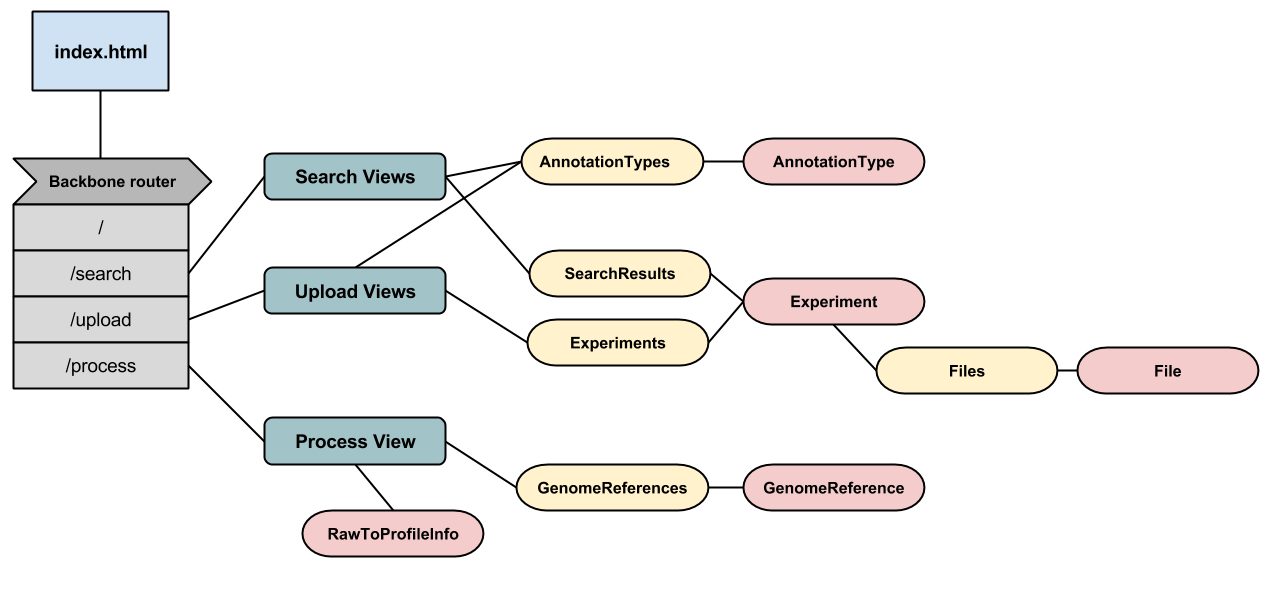
\includegraphics[width=1\textwidth]{web_system_overview.png}
\caption{\label{fig:web_system_overview}Overview of the relations between the different javaScript prototypes in the system.}
\end{figure}

Since our app is built using Backbone\cite{web_1}, our app is divided into the parts \textbf{Misc}, \textbf{Views}, \textbf{Collections} and \textbf{Models}. In \refer{fig:web_system_overview}, we can see the system overview. The \textbf{views} are the parts in green, the \textbf{collections} the parts in yellow and the \textbf{model} the parts in red. The parts in grey represent the router which belongs in our Misc category. It is responsible for rerouting links. For example, when a user clicks the search tab, the router navigates to /search, but instead of loading the whole /search over the page we are currently on, our router will open our search tab below our navigation bar. The \textbf{Misc} category also holds our Main.js, which is in charge of setting up and starting the app.

\subsubsection{Search}
The search tab has three views, the main one being \textit{Search}, which acts as a container for the \textit{SearchResultsView}and holds the search input field and the various buttons displayed. The \textit{SearchResultsView} handles rendering the annotations and the \textit{ExperimentViews}, where one \textit{ExperimentView} is created for every experiment returned from a search. The actual data retrieved is stored, by experiment, in \textit{Experiment models}. To organise this data, we have a collection to contain all the experiments retrieved, called \textit{SearchResults}.
 
%figure bla bla/lalalallala
\begin{figure}[h]
\centering
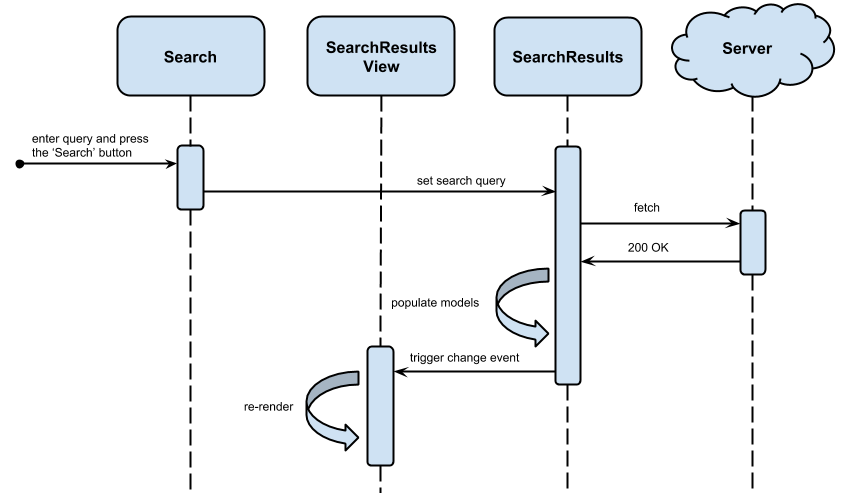
\includegraphics[width=1\textwidth]{web_system_sequenceDiagram.png}
\caption{\label{fig:web_system_sequenceDiagram}a sequence diagram showing what happens when a user enters a valid search query and results are fetched.}
\end{figure}

In \refer{fig:web_system_sequenceDiagram} is a simple sequence diagram for the search tab. If a user enters a query in the search field and then presses the search button, the \textit{Search} view will update the \textit{SearchResults} collection to have a new query. Once \textit{SearchResults} has a new query, it will try to fetch search results corresponding to the query from the server. If successful, new experiment models for every experiment retrieved will be created and set in the \textit{SearchResults} collection. \textit{SearchResults} then triggers a ‘change’ event that \textit{SearchResultsView} listens to. When that event occurs, \textit{SearchResultsView} knows that \textit{SearchResults} has been changed, and re-renders itself.


\subsubsection{Upload}
The upload tab has three main views, the main one being Upload, which acts as a container for the ExperimentView’s and holds the search input field and the various buttons displayed. Each ExperimentView handles rendering the AnnotationsForm and the FileUploadList, where one ExperimentView is created for every experiment the user inputs. The actual annotation data is stored by the \textit{Experiment} model. Files are stored as a \textit{Files} collection in the \textit{Experiment} model. \textit{Experiments} are in turn stored in the \textit{Experiments} collection.
\subsubsection{Process}
Processing has genomeReferences to match with the specie the processing is being done on. Other that that the processing part is mainly a graphical interface with not that much systemDesgin in.

\subsection{System administration - Web}
The system administration part of the web client is developed using the same tools and frameworks as the rest of the web client.
This admin part of the system is made up of view classes, model classes and collection classes. The classes are described below:

\subsubsection*{Classes used by all views}

\strongTerm{Gateway} - this is a model class used solely for communication with the server. It is a static class in the sense that it doesn't have to be created. It only needs to be included and then its functions can be called immediately without having to be instantiated. The gateway class retrieves the URL from the main JavaScript file this way the URL only needs to be declared once. The URL can then be fetched by any class that includes the Gateway class.

\strongTerm{SysadminMainView} - the main view for the admin tab, this view is used together with every other admin view. It contains a sidebar menu used to navigate between different admin views.

\subsubsection*{Classes used to handle annotations}

\strongTerm{Annotation} - this is a backbone model that represents an annotation. An annotation consists of three fields. A name, a list of values and a forced field. The name simply specifies the name of the annotation. The list determines whether this annotation is a drop-down list, or a free-text field. If the list contains one element called free-text, the annotation is a free-text field. Otherwise it is a drop-down list with the values in the list. The forced field determines if
the annotation has to be filled in by the user when a file is uploaded.

\strongTerm{Annotations} - this is a backbone collections that consists of several Annotation models. It also has a URL that it uses to fetch annotations from the server, the URL is retrieved from the Gateway class. 

\strongTerm{AnnotationsView} - this view is the basic view for displaying annotations. It has a search field and a button for creating new annotations. Pressing the button renders the newAnnotationView. 

The AnnotationsView has a child view called AnnotationListView. This way the list view can be rendered separately from the search field when the user types in searches. 

\strongTerm{AnnotationListView} - this view uses the Annotations collection to fetch all the annotations from the server and renders them dynamically in a list.
In the list is an Edit button for every annotation, the edit button will retrieve the name of the desired annotation and navigate through the router to the EditAnnotationView with the name as a parameter.
The view also has a button that will take the user to the NewAnnotationView.

\strongTerm{EditAnnotationView} - this view uses the name parameter received from the AnnotationListView to retrieve a specific annotation from the collection of annotations. It then renders the fields with the values from the annotation. This view has a button to delete an annotation. It will send a delete message to the server using the Gateway model to delete the annotation. An annotation can also be modified in different ways.

\strongTerm{NewAnnotationView} - this view is used to create a new annotation. It consists of a couple of fields and a create button. Pressing the create button renders a ConfirmAnnotationModal which displays the values for the annotation.

\strongTerm{ConfirmAnnotationModal} - this class extends the ModalAC class. It is simply used to display information that the user has to confirm. Pressing confirm creates a message using the Gateway class and sends it to the server.

\subsubsection*{Classes used to handle genome releases}

\strongTerm{GenomeReleaseView} - this view is used for viewing, adding and deleting genome releases. It contains a button ''Select files to upload'' which opens up file explorer and lets the user select one or multiple files for uploading. When the user then presses upload the UploadGenomeReleaseModal will open. Below the button the view has a table showing the current genome releases available on the server. The user can hold the mouse over files too see all files included in that genome release. A ''Delete'' button is shown next to every genome release and if pushed sends a delete request to the server through the Gateway class. 

\strongTerm{UploadGenomeReleaseModal} - this modal shows the user which files has been selected for upload and asks for information about which species and genome version they are for. Then at the press of ''Upload'' the files starts to upload and the user will see a progress bar over the complete upload progress. 

\strongTerm{GenomeReleaseFiles} - this is a collection with GenomeReleaseFile as models. It handles the ordering and filtering of its models. 

\strongTerm{GenomeReleaseFile} - this model represent a genome release and can contain multiple files in itself since one genome release is almost never just one file. This class takes case of uploading itself to the server and thereby also updates the progress bar through events that propagate up to the GenomeReleaseFiles collection. 

\FloatBarrier

\section{Android application}
The following sections describe the system design of the Android application. All functionality of the system components are described in this section. Worth noting is that the figures referred to in this section can be found further down in the document.

\subsection{System overview}
	The Android application is divided into seven \emph{packages}. These packages are \verb!default!, \verb!com!, \verb!login!, \verb!model!, \verb!process!, \verb!processStatus! and \verb!search!.
	All packages (except for \verb!com! and \verb!model!) contains one or several fragments. A \verb!Fragment! is an object that helps to modularize the code and brings more sophisticated user interfaces.

	\begin{figure}[h]
		\centering
		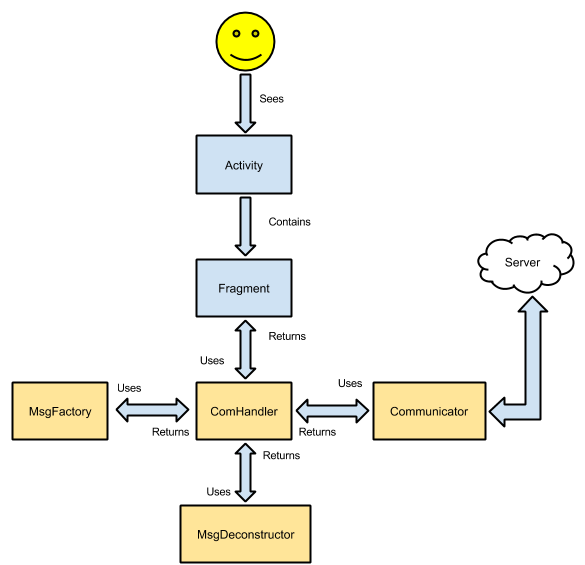
\includegraphics[width=1\textwidth]{and_system_overview.png}
		\caption{\label{fig:and_system_overview}A generalization of how the Android application works.}
	\end{figure}

	The user will interact with an activity that holds a fragment. The fragment (which contains some logic) will tell the class \verb!ComHandler! what action that should be performed. The \verb!ComHandler! will construct a message by using \verb!MsgFactory!. The message is then passed on to \verb!Communicator! which sends the message to the server with REST. The \verb!Communicator! returns the response to the \verb!ComHandler! that parses it by using the class \verb!MsgDeconstructor! and then returns it to the fragment. Hopefully, \refer{fig:and_system_overview} will bring some clarity.
	
\subsection{Package overview}
	The \verb!default! package contains the \verb!MainActivity!. This class is the base of every screen in the application after logging in. The top level navigation is handled from here.

	The \verb!com! package is responsible for communication with the server. It also contains classes and methods for construction and deconstruction of JSON.

	The \verb!login! package contains the GUI and controller for the login screen. It also enables the user to select, add, edit and delete server URLs.
	
	The \verb!model! package holds information about experiments, annotations, files etc. found on the server.
	
	The \verb!process! package is responsible for displaying processing parameters etc. for when the user wants to start a process.

	The \verb!processStatus! package shows the running, failed and succeeded processes on the server.
	
	The \verb!search! package handles searches by either selecting annotations, or by manually typing in PubMed style. It also handles the search results by displaying the found experiments in a list.
	
\pagebreak


\FloatBarrier

\section{iOS application}
The following sections describes the system design of the iOS application. The overall system design is discussed followed by a more detailed description of how the segues are controlled.

\subsection{Overall system design}
The  system is designed using the model-view-controller principle. Each view is controlled by its own controller class which reacts to user input and triggers changes in the model and updates the view accordingly.
\begin{figure}[ht]
\addScaledImage{0.3}{ios_UML2.png}
\caption{UML diagram.}
\label{fig:ios_UML}
\end{figure}
\FloatBarrier

\refer{fig:ios_UML} gives an overall image of the system design. Some classes are excluded from the figure to make it easier to get an overall idea of the system. The controller classes of the table cells and some other controller classes are not illustrated in the diagram. The non-excluded classes are described in \refer{table:ios_class_table}.

\begin{table}
\begin{tabularx}{\textwidth}{|l|X|}
\hline
\textbf{Class} & \textbf{Description} 
\\ \hline
\term{Annotation} &
Contains information about an annotation and can format the annotation name to an aesthetically more pleasing representation.
\\ \hline

\term{DataFileViewController} &
Controls the File view presented in \refer{fig:ios_files1}. It contains a reference to an experiment and lists all its files in a table.
\\ \hline

\term{Experiment} &
A class that contains information related to an experiment, as well as its files.
\\ \hline

\term{ExperimentDescriber} &
Generates a description of an experiment using annotations chosen by the user.
\\ \hline

\term{ExperimentFile} &
Contains information about a file from an experiment.
\\ \hline

\term{ExperimentParser} &
Parses experiment information from a NSDictionary to an Experiment object.
\\ \hline

\term{FileContainer} &
Contains files and sorts them by file type.
\\ \hline

\term{JSONBuilder} &
Creates different JSON requests.
\\ \hline

\term{PubMedBuilder} &
Creates a pubmed search query.
\\ \hline

\term{SearchResultController} &
A controller class for the Search Results view presented in  \refer{fig:ios_searchResult}. It configures the table which holds the information about the experiments a search resulted in. An ExperimentDescriber is used to generate a description of the experiments.
\\ \hline

\term{SearchViewController} &
A controller class for the Search view, see \refer{fig:ios_search}. It checks which annotation-fields are used and tells the JSONBuilder to generate a corresponding search query when the user presses the search button. The class also contains a advanced search to allow the user to manually enter search queries. 
\\ \hline

\term{SelectedFilesController} &
A controller class for the The selected files view shown in \refer{fig:ios_selectedFiles1}. The selected files controller contains information about files saved by the user.
\\ \hline

\term{ServerConnection} &
Sends and receives JSON objects to and from the server.
\\ \hline
\end{tabularx}

\caption{Description of some classes of the system.}
\label{table:ios_class_table}
\end{table}
\FloatBarrier

A more detailed description of these classes, and the ones not mentioned here, can be found in comments in the source code.

\subsection{Segue controll}
To avoid several segues to be executed at the same time, a segue controll package has been implemented. Instead of extending UIViewController, UITableViewController, UITabBarController and UINavigationBar the corresponding XYZ class should be used instead. An overview of this design can be seen in \refer{fig:ios_UML_segue}. This figure also includes the classes XYZDataFileController and XYZSearchResultController as two examples of such implementations.

\begin{figure}[ht]
\addScaledImage{0.35}{ios_uml_segue2.png}
\caption{UML diagram describing the segue controll.}
\label{fig:ios_UML_segue}
\end{figure}
\FloatBarrier


\FloatBarrier

\section{Server}
The system design of the different parts of the server.
\subsection{Communication}
\subsection{Communication}
The server is based around HTTP, where clients send requests on a non-persistent connection and the server responds to these requests. All communication is initiated by the client and the server has no way of contacting clients except when responding to a request. 

Clients send requests to the communication part of the server first. When a request is recognized by the server, the request is parsed and a command is created depending on the request. The command then communicates with the other parts of the server in order to extract or input relevant data. 

To identify clients a unique token is used, which is generated when a user logs in. The token is sent back to the client, and the client must include this token with all following requests. Since there is no persistent connection between the client and the server this token is the only way for the server to identify the sender for any given request. The token is also used to prevent unauthorized requests from being executed on the server.

Most commands are executed immediately when the server gets a request, and the result is sent back to the client when the command is finished. This happens when for example searching the database. 

The commands implemented for the server are:

\begin{itemize}
	\item $login$
	\item $search$
	\item $annotation$
	\item $experiment$
	\item $file$
	\item $process$
	\item $genomeRelease$
\end{itemize}

The $login$ command can take either a $'POST'$ method or $'DELETE'$ method, depending on if the user wants to log in or log out. 

$search$ is used for searching for experiments in the database. Results will display all experiments which match the search query, and the user can chose o expand these experiments in order to view the containing files. 

The $annotation$ command can be used to modify and view annotations associated with experiments. The server can respond to a $'GET'$ request with an array of all possible annotations currently in use in the database. There is also possible to add new annotations, update the values for an annotation or delete a complete annotation field. 

Clients can get information about a specific $experiment$ by using a $'GET'$ together with this command. The server will respond with information about the experiment aswell as information about all the files associated with the experiment. Clients can also add, modify and delete experiments. 

An experiment contains $file$s which can be uploaded with this command. A $'POST'$ will let the client upload a file to a specific experiment. Clients can also download, modify and delete files. When a client downloads a file, the communication part of the server is never contacted. This is because a download URL is already present in the file on the client side. Therefore no contact is needed with the communication part of the server, but instead the file system server takes care of the request. 

In order to convert files, the client can send the command $process$ together with a $'PUT'$. This will convert specific raw files into profile files. If the client instead sends a $'GET'$ it will recieve a list of all processes started, and their remaining time until completion. 

$genomeRelease$ can be used to edit genome releases, these files are then used when converting files. The client can specify to convert a file from one genome release to another, if it exists in the database. 

A more detailed specification of the API can be found in the appendix. 
\FloatBarrier
\subsection{Data Conversion}
The Genomizer service needs to be able to convert, process and visualize data. This chapter explains how this is done in the system.

\begin{figure}[h]
\addImage{UMLsprint2.jpeg}
\caption{Classdiagram for Process}
\label{con_UML}
\end{figure}
	
As can be seen in \refer{con_UML} the RawToProfileConverter extends the Executor class. When a call comes to the ProcessHandler it then starts the correct convertion which right now only can be a raw to profile conversion.


\subsubsection{Executor}
The executor class, as seen in figure 5.2.1, is a abstract superclass that is an entity that is able to execute various commands. The executor class is able to run programs as well as scripts and shell commands. In order to run scripts and programs the executor has a parse-function that parses a string into separate arguments. \newline

\begin{itemize} 
\item executeCommand
\begin{itemize}
\item ExecuteCommand is a private method that is being used by the executeScript, executeProgram and executeShellCommand methods. Firstly a processBuilder is used to ensure a safe way to execute commands, after that the working directory is set and the error output stream is merged with the standard output.
After a command has been started the output stream is then recorded with the help of a scanner object and a stringBuilder object. When the command has been executed the recorded string is sent back to the caller.
\end{itemize}
\item executeScript/executeProgram
\begin{itemize}
\item Both methods are very similar. The difference is that executeScript has a static filepath added to the second argument. This is because the first argument when calling a script is the script language instead of the actual script file. E.g. shell resources/script.sh.
\end{itemize}

\item parse
\begin{itemize}
\item In order to receive a command string and to be able to run it a parse method had to be implemented. This is because the processbuilder takes a String array as argument. With the help of a tool called stringTokenizer the string is parsed into a String array separated on spaces.
\end{itemize}
 
\item cleanUp
\begin{itemize}
\item Recieves a stack with folder names as strings and removes the folders files and then the folder itself. Used to clean up after a process have been executed and generated files during the procedure. 
\end{itemize}

\end{itemize}

\subsubsection{RawToProfileConverter}
\emph{The purpose of the RawToProfileConverter class is that it will be used by processHandler and do all the different steps needed to make a raw file. These steps are done by using the program Bowtie and by running two different scripts which are executed with methods that is extended from Executor class. When ratio calculation is supposed to be done, there are 2 more steps that will be done.}

\subsubsection{Description of Procedure}

\begin{enumerate}
\item Bowtie: Creates unsorted .sam files. Puts the files in a created temp folder with the name result\_X, where X is the number of the current thread. All other folders created is placed inside the folder from where the files used where placed.
\item sortSam: Sorts the .sam files and creates new .sam files. Puts the files in a folder called sorted.
\item Run Gff: Processes the sorted sam file and creates a gff3 file. Puts the files in a folder called reads\_gff.
\item Allnucsgr: Processes the gff3 file and creates a sgr file. Puts the files in a folder called allnucs\_sgr.
\item Smooth: smooths the file and creates a large .sgr file, converted the customers perl script by following the algorithm they  sent us. This makes it more efficient. Puts the files in a folder called smoothing.
\item Step: Takes the smoothed .sgr file and takes samples from it with a specified intervall and creates a smaller .sgr file. If stepping is done the files will be placed in the same folder as the previus step.
\item Ratio Calculation: Creates four .sgr files with the perl script provided by the customer. Puts the files in a folder called ratios.
\item Smooth: After the ratio calculation, smoothing needs to be done again with different parameters. Puts the files in a folder called smoothing
\end{enumerate}


\begin{itemize} 
\item procedure
\begin{itemize}
\item Executes all the steps to make a profile .sgr file from a raw file, it checks the directory it gets as filepath so that it contains the raw files and that there arent more then two files, but atleast one file to process. Does the procedure to create a profile data and move it to the folder thats specified as a parameter.
\end{itemize}

\item runBowtie
\begin{itemize}
\item Constructs a long string with the full execution line for bowtie. It then uses this string as a parameter when calling the method parse. 
The resulting array is then used when calling executeProgram and the result of the execution is returned.
\end{itemize}
\item sortSamFile
\begin{itemize}
\item Constructs a string with the full execution line to sort a sam file. It then calls parse to create a string array from the full string and sends it as parameter to executeShellCommand which runs a shell command to sort the file and creates a new .sam file that is sorted with the specified parameters.
\item makeConversionDirectories
\begin{itemize}
\item Creates the necessary directories used by RawToProfile's procedure to put the temporary files needed to do all the steps to create a profile .sgr file.
\end{itemize}
\item initiateConversionStrings
\begin{itemize}
\item Defines all strings needed for the directories created when procedure is doing its work. Also defines a string for each step in the procedure, which gets passed to the corresponding execute methods. 
\end{itemize}
\end{itemize}
\end{itemize}

\paragraph{Bowtie}
Bowtie takes two raw .fastq files and converts them to .sam which is the first step to make the desired .sgr files. After a .sam file is converted the linux command sort is run  on both files which creates two sorted .sam files, it is sorted by chromosome and position as needed to use the scripts.
\paragraph{Used scripts}
The different functions of the perl scripts is explained below. They are explained in the same order that they are executed. All scripts take a directory of files to be processed as input parameter.

\begin{itemize}
\item[samtoreadgffv1] Makes a .gff file from a sorted .sam that have reads at each nucleotide positions. No input parameters except the directory of the sorted sam files are needed. The resulting files are put in the new folder \textit{reads\_gff}.

\item[readsgfftoallnucsgrv1]  Counts the reads from the previous script result. For each chromosome reads are read and each nucleotide position is incrementally counted with one when a read cover it. No parameters are needed for this script except the file path of the gff files. The resulting files are put in the new folder \textit{allnucs\_sgr}.

\item[ratio\_calculation\_v2] Does ratio calculation on the processed files. For each position in the IP sample with at least one mapped read, a ratio of IP-input(on a log2 scale) is calculated. If the read count in the input is below the read -count mean (in the input sample) is calculated it is set to the mean( or double mean (2 x mean) as user specifief). If the input mean is below four the minimum input value is set to four (to avoid division by nearzero values; calculated as -(read lenght x approximate total number of reads in input samples(9 millin))/ genome size (for Drosophila melanogaster 120381546)). A random number between -0.5 and 0,5 is added to the read counts before log2 conversion to make them discrete for statistical analysis. All ratio values are then adjusted by reducing each value by median of the ratios. This linear adjustment is carried out in order to compensate for differences in IP and input sequencing depth. Also, to visualize ratios distribution, ratios are plotted by binning ratios with user specified numbers of bins and minimum and maximum ratio values(200bins,minimum ratio value: -10, maximum ratio value:10). Ratio values are printed in sgr format.
 

\end{itemize}

\subsubsection{Smoothing and stepping}
\emph{The scripts that was provided was inefective and in order to reduce ram usage and getting faster Raw-To-Profile conversion we rewrote the smoothing and step scripts into a built-in solution in the java server.}

\paragraph{SmoothingAndStep}
Smoothing means that we either calculate the trimmed mean value or median value for a position and a number of proceeding positions. The number of positions we should smooth on is called the Window Size. We also need to have a cutoff number, which tells us that if we have fewer rows to calculate on than the cutoff number we shouldn't smooth at all. There's also one parameter called stepSize, if the stepSize is one the program will not do any stepping but if it's larger than 1 stepping will be done. Stepping is handled in this program by simply checking every time we are going to write to the new file if the current row's position is divisible with the stepSize, if it is we write to the file, otherwise the row is discarded.

The class SmoothingAndStep have one public method and many private ones. The public one called smoothing starts by setting up file readers/writers. It then reads as many rows from the file as the window size. It then smooths one row. From then on the program removes the first row from the array and add one new row to the array and then smooth the first one in the array. This continues until either we start closing in on the end of the file or when we come close to a chromosome shift. These special cases are handled a bit different.




\paragraph{Tuple}
The tuple class is a data carrier that represents one row of data in an sgr file. It consists of the fields chromosome, position, signal and newSignal. Where signal is the signal-value read from the infile and newSignal is the updated value after smoothing have been done.
The methods in this class are all standard getters/setters except for the method toString which formats a row for the outfile and rounds of decimal numbers. The constructor is also of interest since it parse a row on tabs. Thus the fields in an infile needs to be seperated by tabs and not spaces.


\subsubsection{ProcessHandler}
The processhandler is a controller that handles process-calls. Depending on the name of the process it handles it differently. It acts as an interface between the process-module and the rest of the program. 


\subsubsection{Logic \& interface}
The main logic in the processHandler is a switch-case that switches on the name of the process being called. For example if the name of the process is “RawToProfile” is sets up a RawToProfile-converter and calls it. 

\begin{itemize}
\item[processName] A string that tells the handler which kind of process should be executed.
\item[procedureParams] A list of string with the parameters to the different external  programs/scripts that will be called during the execution. The first element will be a string with parameters/flags for the first external program that will be called, and so on.
\item[inFile] A string with a path to the directory containing the files that should be operated on.
\item[outFile] A string with a path to the directory where the result .sgr files should be put.

\end{itemize}





\FloatBarrier
\subsection{File-transfer}
In the current version of the program the desktop clients and the web clients connect to different software on the server for communication. The desktop clients connect directly to the server communication software whilst the web clients connect via the apache server and all non web requests that is to be calculated using the server software is automatically redirected by apache.
The redirect is setup in a way that all GET requests that have a /api/ tag in the URL will be redirected.
The exception for the desktop clients are file up- and downloads which are done through the apache server.

The download and upload will work for all platforms although this will not be implemented for Android and iOS clients due to hardware limitations.

If the client wishes to upload a file to the server they first send a request to the server-system which authenticates the client and stores the annotations for the file. The download and upload path is validated by the script so no invalid paths are sent to the scripts.

For uploading and downloading files via Apache, two PHP-scripts will be used. If the user wants to upload a file, the PHP-script will try to store the file in a location on the server provided by the client. A script for downloading files from the GEO database and saving them on the server is currently being  implemented, although not yet fully tested nor implemented by the clients. See \refer{chap:servercmd} for examples when using the PHP-scripts.

In \refer{fig:exp_flow} below it is shown how the systems handles the different types of messages the client-systems can send. The big square represents the Apache server with different parts of the Apache server within. The iOS and Android clients can only send some requests to some computation to the server-system. Meanwhile the desktop client can send requests to the server-system and upload and download to/from the web server. The web client sends all its messages to the Apache server and if it is a request to do some sort of computation it will be redirected to the server-system and if it is a download, upload or web-page message it will be sent to the web server.

\begin{figure}[hbt]
\addImage{exp_flow}
\caption{A figure showing the different types of messages sent between the systems.}
\label{fig:exp_flow}
\end{figure}

The current version of the system utilizes a file structure to organize HTML- and file requests on the server, the structure is illustrated in \refer{fig:exp_filestructure}. The Web-root folder houses the PHP-script for uploading and downloading files. The app folder contains the \appName\ web page. In the data folder are all the experiments folders, which contains folders for the different data-types.

\begin{figure}[hbt]
\addImage{exp_filestructure}
\caption{Figure illustrating the current file tree on the server machine.}
\label{fig:exp_filestructure}
\end{figure}

\FloatBarrier
\subsection{Database}
\section{System Design}

Our system for the file storage is basically built up with a database and a file system, where the header information of a file is stored in the database and the real file is stored in the filesystem. A filepath string is stored in the database as “path”, so the user can find where the actual file is stored in the filesystem. You can see the database design in the schema below (\refer{fig:dat_databaseSchema} ). \\
\\
Note that this section only describes the advanced system design that needs further explanation than just reading the code. Also note that it exists some javadocumentation that explains all methods in each class further deeper and more specific than this documentation that might be useful for those that will continue developing this system. Those can be found in the same file directory as the program, in the sub dir "/doc".

\begin{figure}[htb]
\addImage{dat_schema_V3.jpg}
\caption{Schema for the database.}
\label{fig:dat_databaseSchema}
\end{figure}

\FloatBarrier

\underline{Comments about the database design:}\\
\\
* FileID is a unique number for a specific file. It will be autogenerated by the database when you insert one file row.\\
* Path is where the actual file is stored in the filesystem, example:\\
\\
\centerline{$home/data/experiment_1/raw/rawFile1.raw$}\\
\\
Since many files are stored in pairs, the InputFilePath is the path to where the other file pair  is stored.\\
* MetaData is the arguments used when converting. \\
* IsPrivate is a boolean (T or F) for making the file private or not.\\
* Role in User Info determines the user rights for one user in the system, examples could be admin, user, etc.\\
"Annotated With" is the table that connects one experiment to one annotation, example:
\begin{center}
  \begin{tabular}{| l | l | l | l|}
    \hline
    $Experiment_1$ & Species & Dog\\ \hline
  \end{tabular}
\end{center}
* "Annotation" is the table containing the annotation with a preset default value, but not any choices. example:
\begin{center}
  \begin{tabular}{| l | l | l | l|}
    \hline
    Species & DropDown & Human & T \\ \hline
  \end{tabular}
\end{center}
"Annotation choices" is the actual values for a specific annotation, example:\\
\begin{center}
  \begin{tabular}{| l | l | l | l|}
    \hline
    Species & Dog \\ \hline
    Species & Fly \\ \hline
  \end{tabular}
\end{center}
* The "Genome Release" table stores information about each stored genome release file, but the "Genome Release Files" table stores information about its convertion status, which at the moment could be "done","processing", "Pending", "Aborted". This table only exist for the Gui to being able to keep track of all the queued convertions.\\
* The "Chain File" table keep information about stored chain files, and the "chain file files" table stores information about all the current queued chain convertions.\\
NOTE: The tables "Working On", "Workspace", "Used In", and "Publihed in" has not been implemented yet but is planned to exist in the final version of the program. Those tables are used to connect files to a workspace of a user or users. But the connection is only a reference to where the file is actually stored. 

\subsection{System overview:}
The datastorage part of the system is built up of many classes that work together, but there is only one class that connects all subclasses and should be used by other parts of the genomizer program. This "front door" class is called "DatabaseAccessor.java". On the next page there are two uml diagrammes visible (\refer{fig:dat_umlPart1} and \refer{fig:dat_umlPart2} ) that describes all the classes in the datastorage system and how they are connected to each other.

\FloatBarrier
\newpage
\begin{figure}[H]
\addImage{dat_Uml3_part1.jpg}
\caption{The first part of the UML diagramme for the datastorage part of the genomizer program.}
\label{fig:dat_umlPart1}
\end{figure}

\FloatBarrier

\newpage
\begin{figure}[H]
\addImage{dat_Uml3_part2.jpg}
\caption{The second part of the UML diagramme for the datastorage part of the genomizer program.}
\label{fig:dat_umlPart2}
\end{figure}

\FloatBarrier

\newpage
\subsection{Method description:}
Below is some interaction processes described and what happens in the databaseAccessor class that needs further description than just viewing the class or the javaDoc.\\
\\
\underline{GetExperiment:} Will find a specific experiment from one experimentID, from the database and will return an experiment object for that experiment. The object will contain information about the experiment id, experiment annotations connected to that experiment, and all files connected to that experiment with their headers. The object contains both setter and getter methods. \\
\\
\underline{Adding one experiment step by step:}
There are some steps that need to be done in the right order to be able to add one experiment into the database. The order is as follows:\\
\\
1: First you will need to call the "addExperiment" method. It will add one experiment to the database witout any annotations set to that experiment. If you try to add one experiment that already exist then the addition will be refused and one exception will be thrown.

2: Then you add the annotations in general that should exist in the database.This can be done in many different methods depending on what purpose the annotation should have. Those are:\\
\\
a) AddFreeTextAnnotation: adds a free text annotation that will not be visible as a dropdown choice for the gui. Example for one entry line in the database could be: "Tissue,FreeText,Null,T".\\
\\
b) AddDropDownAnnotation: adds one annotation that will be visible as a dropdown choice for the gui. This method wants the label and a list of all annotation choices that the label should have, and also a default value. This method will fail if that annotation already exists in the database. Example of one entry could be: "Sex, DropDown, Male, T".\\
\\
c) AddDropDownAnnotationValue: If the method above fail because that annotation already exist in the database, you can run this method to just add one annotation choice to one existing annotation label, example: "species,dog".\\
\\
3: Once the annotation is set, you can connect the experiment with the annotations. This is done by calling the method "annotateExperiment". It is also here the FreeText annotations stores its values.\\
\\
Now the experiment should be in the database with annotation values, and is now ready to have files added to it.\\
\newpage
\underline{Get methods:}\\
\\
* GetChoices: Gets you all the available annotation choices connected to one label that you send in as inparameter. Example is "sex" that might return a list with values "Male,Female,Unisex,Unknown".\\
\\
* GetAnnotations: returns all annotation labels currently stored in the database. Examples could be "Sex,Species,Tissue,etc.".\\
\\
* GetAllAnnotationObjects: Does the same as the method GetAnnotation, but return it as an arrayList instead.\\
\\
* GetAnnotationObject: one method where you send in one label and get back one annotation object containing the "annotation" row  from the database, aswell as all its connected annotation choices.\\
\\
* GetAnnotationObjects: Same as getAnnotationObject but it returns a list of annotation objects from a list of annotation labels.\\
\\
\\
\underline{Change Methods:}\\
\\
* ChangeAnnotationLabel: changes one entire label in the database.\\Example: "Sex, Tissue, etc.".\\
\\
* ChangeAnnotationValue: change one value for a specific annotation label.\\Example: "male,female,fly,etc.".\\
\\
* UpdateExperiment: Updates one annotation for one specific experiment. Example: "experiment1, species, human" can be changed to "experiment1, species, Fly". Note that the new label must exist in the "Annotation" table.\\
\\
* ResetPassword: reset the password for one user to a new password. \\
\\
\underline{Remove methods:} All the remove methods will delete both the database entry and the physical files when called. These are the following remove methods that exist:\\
\\
* DeleteAnnotation: Deletes an entire annotation from the database. Since the database is configured to delete on cascade, all annotation choices connected to that annotation label will be removed, also the connection to the experiments with that annotation label.\\
\\
* RemoveAnnotationValue: Removes a single annotation value connected to a label, for example: "fly", or "arm".\\
\\
* RemoveGenomeRelease: Removes a whole genome release. But you must first make sure that all files using that genome releases is deleted so no databae dependenies exist. Also you must first delete the entries for that speific genome release in the tables "Genome Release Files", "Chain File" and "Chain File Files". This is done by calling the methods "RemoveReleaseFiles", "RemoveChainFile" or "RemoveChainFileFiles" respectively. \\
\\
* DeleteFile: deletes both the entry for a file and the actual data from the server. This can be done by two methods with different parameters,the first by file path, the other by fileID.\\
\\
* DeleteUser: delete one user from the database and he or she will not be able to use the program any more.\\
\\
\underline{Adding files:}\\
To add a file you will need to have an experiment added before you call the "addNewFile" method. Some files uses multiple files like raw data so make sure that you upload them together and that the "InputFilePath" points to their other file pair.\\
\\
\underline{Removing files:} Also here, if you delete one file that comes as an file pair, you must also delete the other file thorugh this method.\\

\underline{Other:} There exist other methods as well, but these does not need any further description then what is written in the java class DataBaseAccessor.\\
\FloatBarrier
\subsection{Apache}
The Apache HTTP Server or commonly referred to as Apache, is the web server application that was decided to be used to upload and download files to and from the server. Apache is open source, that makes it free to use. Apache is a good choice because it is developed and maintained by an open community, that way all new versions and updates will become available for free. And since it is open source, the source code is open for everyone to read. Apache can be used on both Unix/Windows systems, but in this case it is currently running on a Unix machine but can still communicate with all platforms. 

\subsubsection{Server user manual}
The Apache server is controlled from the terminal, this can be done either directly from the server or remotely from another computer using SSH. To use SSH from another computer, write

\texttt{ssh username@address.to.server}

in the terminal, when asked for password enter the password for the server. Then write the commands directly in the terminal.

These are some of the most common commands for apache: \\
\begin{tabular} {| l | l |}
\hline
\textbf{Action} & \textbf{Command} \\
\hline
Start Apache & \texttt{sudo service apache2 start} \\
\hline
Stop Apache & \texttt{sudo service apache2 graceful-stop} \\
\hline
Restart Apache & \texttt{sudo service apache2 graceful} \\
\hline
\end{tabular}
\FloatBarrier
